\documentclass[final]{beamer} % beamer 3.10: do NOT use option hyperref={pdfpagelabels=false} !
  %\documentclass[final,hyperref={pdfpagelabels=false}]{beamer} % beamer 3.07: get rid of beamer warnings
\mode<presentation> {  %% check http://www-i6.informatik.rwth-aachen.de/~dreuw/latexbeamerposter.php for examples
	\usetheme{JK2}    %% you should define your own theme e.g. for big headlines using your own logos 
}

\setbeamertemplate{caption}[numbered] 
\usepackage[english]{babel}
\usepackage{framed}
\usepackage[utf8]{inputenc}
\usepackage{amsmath,amsthm, amssymb, latexsym}
\usepackage{booktabs} % nice tables
\usepackage{multirow}
\usepackage{sidecap}
\usepackage{soul}
\usepackage{setspace}
\usepackage{changepage}
\usepackage{csquotes}

\newcommand{\mr}[2]{\multirow{#1}{*}{#2}}  
\newcommand{\mc}[3]{\multicolumn{#1}{#2}{#3}}  

\newcommand{\tcb}[1]{\textcolor{blue}{#1}}
\newcommand{\tcr}[1]{\textcolor{red}{#1}}

%\usepackage{times}\usefonttheme{professionalfonts}  % times is obsolete
%  \usepackage[absolute,overlay]{textpos}
% \usefonttheme[onlymath]{serif}
\boldmath
\usepackage[orientation=portrait,size=a0,scale=1.4,debug]{beamerposter}                       % e.g. for DIN-A0 poster
%\usepackage[orientation=portrait,size=a1,scale=1.4,grid,debug]{beamerposter}                  % e.g. for DIN-A1 poster, with optional grid and debug output
%\usepackage[size=custom,width=200,height=120,scale=2,debug]{beamerposter}                     % e.g. for custom size poster
%\usepackage[orientation=portrait,size=a0,scale=1.0,printer=rwth-glossy-uv.df]{beamerposter}   % e.g. for DIN-A0 poster with rwth-glossy-uv printer check
% ...
%
\title{Analytical and Monte-Carlo modeling of Multi-Parallel Slit and Knife-Edge Slit Prompt Gamma Cameras}
\author{E. Testa\inst{1}, B.F.B. Huisman\inst{1,2}, D. Dauvergne\inst{3}, J. M. L\'etang\inst{2}, D. Sarrut\inst{2}}
\institute[]{
	\inst{1} Universit{\'e} de Lyon, Universit{\'e} Claude Bernard Lyon 1, CNRS/IN2P3, Institut de Physique Nucl{\'e}aire de Lyon, 69622 Villeurbanne, France, \inst{2} CREATIS, Université de Lyon; CNRS UMR5220; INSERM U1044; INSA-Lyon; Université Lyon 1; Centre Léon Bérard, Lyon, France, \inst{3} Universit\'e Grenoble Alpes, Laboratoire de Physique Subatomique et de Cosmologie, CNRS/IN2P3, Grenoble, France}
% \footer{
\includegraphics[height=0.025\textheight]{./figures/logo_IPNL}
\includegraphics[height=0.025\textheight]{./figures/logo-creatis}
\includegraphics[height=0.025\textheight]{./figures/Logo_LPSC}
\includegraphics[height=0.025\textheight]{./figures/logo_primes}\\ Labex PRIMES ANR-11-LABX-0063. \hfill contact: \url{e.testa@ipnl.in2p3.fr}}

\begin{document}
	
\begin{frame}{} 
\vfill
  
%%%%%%%%%%%%%%%%%%%%%%%%%%%%%%%%%%%%%%%%%%%%%%%%%%%%%%%%%%%%%%%%%%%%%%%%    
\begin{block}{1. Introduction}
	\begin{columns}[t]
		\begin{column}{0.49\textwidth}
			\centering{\Red{\large{Ion-range verification during hadrontherapy}}}
			\begin{itemize}
				\item Major challenge to fully take benefit from ion beam ballistic properties
				\item Main imaging modalities under study:  prompt gammas (PG) detection \cite{Krimmer2017a} with non-imaging systems (such as PG Timing, PG Spectroscopy and PG Peak Integral) and imaging systems, namely physically-collimated or electronically collimated cameras (Compton cameras)
			\end{itemize}
		
		\end{column}

		\begin{column}{0.49\textwidth}
			\centering{\Red{\large{PG collimated cameras}}}
			\begin{itemize}
				\item 2 main collimator configurations: Multi-Parallel Slit (MPS) \cite{Pinto2014} and Knife-Edge Slit (KES) collimators \cite{Smeets2012} (Figure~\ref{MPS-KES_scheme})
				\item No theoretical considerations have been proposed for the specific 1D collimation systems developed for PG detection 
			\end{itemize}			
		\end{column}
	\end{columns}

\end{block} % introduction
%%%%%%%%%%%%%%%%%%%%%%%%%%%%%%%%%%%%%%%%%%%%%%%%%%%%%%%%%%%%%%%%%%%%%%%%

\begin{columns}[t]
	
	\begin{column}{0.49\textwidth}
	  \vspace{-2ex}
	  %%%%%%%%%%%%%%%%%%%%%%%%%%%%%%%%%%%%%%%%%%%%%%%%%%%%%%
	  \begin{block}{2. Objectives}
			\begin{itemize}
				\item Development of an analytical model (AM) of MPS and KES collimations $\Rightarrow$ main intrinsic features of each collimator
				\item Verification of the AM by means of Monte Carlo (MC) simulations 
				\item Comparison the MPS and KES prototypes developed by the CLaRyS collaboration \cite{Pinto2014} and IBA \cite{Smeets2012}, respectively.
			\end{itemize}				    
	  \end{block}
		
	  %%%%%%%%%%%%%%%%%%%%%%%%%%%%%%%%%%%%%%%%%%%%%%%%%%%%%%
	  \begin{block}{3. The Analytical Model of MPS and KES collimations}
			\vspace{-10mm}
			\begin{columns}[t]
				\begin{column}{0.5\textwidth}
			\begin{figure}
							\vspace{-10mm}
				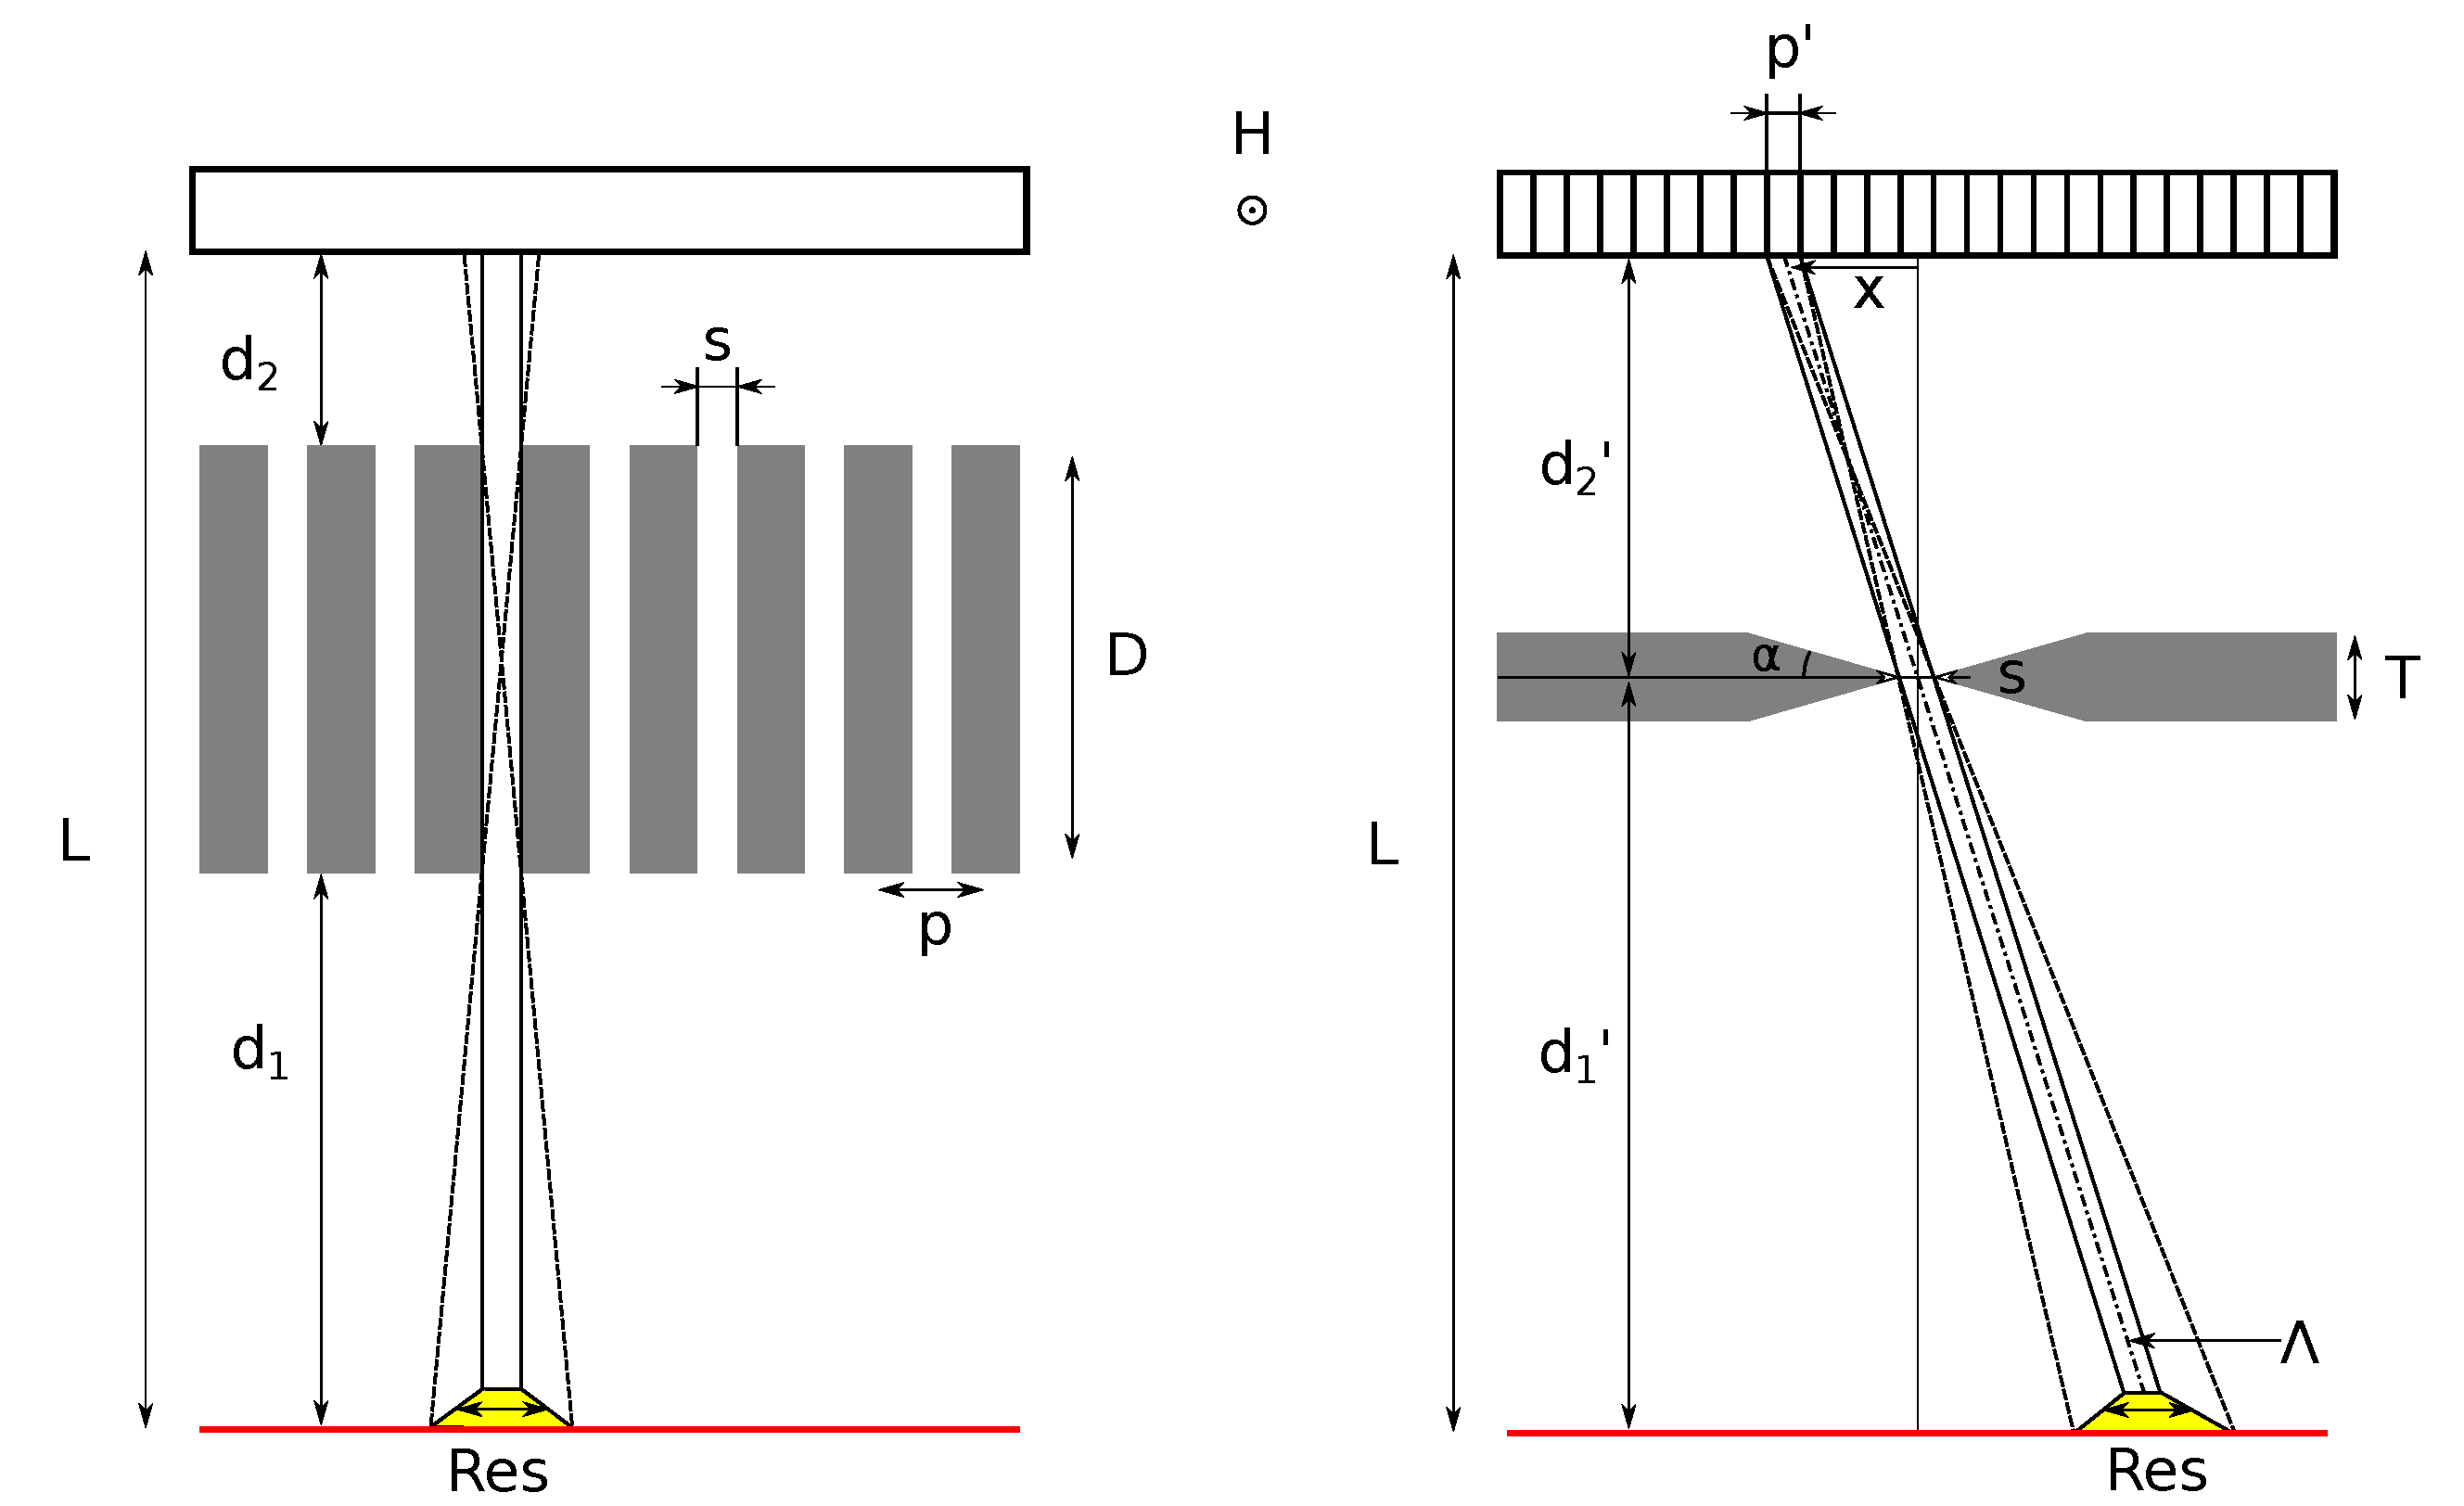
\includegraphics[width=\textwidth]{./figures/MPS-KES_scheme}
				\caption{MPS (left) and KES (right) collimation. $H$: height. $f$: filling factor $((1-s)/p)$}
				\label{MPS-KES_scheme}
			\end{figure}
			

					
				\end{column}

				\begin{column}{0.49\textwidth}
					
					\begin{table}[h]
					\small
					\centering
					\begin{tabular}{lcc}
						\midrule
																				& MPS                              & KES \\
						\midrule
						$s_e$& $s$                              & $s + \frac{\ln(2)}{\mu~\tan(\alpha)}$ \\
						FOW		& $s \left(1+\frac{d_1}{D}\right)$ & $s_e \left( 1+\frac{d_1^{'}}{d_2^{'}} \right)$ \\
						DE	& $\frac{H s}{ 4 \pi L D } (1-f) $ & $\frac{H s_e}{ 4 \pi L d_2^{'} } \left( 1 + \frac{x^2}{d_2^{'2}} \right)^{-3/2} $ \\
						$T_e$ & $D\times f$           & $T$ \\
						\midrule
					\end{tabular}
					\caption{Detection efficiencies (DE) and spatial resolution (Res=FOW) predicted by the analytical model. FOW: Fall-Off Width of the PG profile (see section~ \enquote{Figures of merit}) ; $s_e$: effective slit width ; $T_e$: effective thickness.}
					\end{table}
					
				\end{column}
			\end{columns}
	  \end{block}
	  %%%%%%%%%%%%%%%%%%%%%%%%%%%%%%%%%%%%%%%%%%%%%%%%%%%%%%
		
	  \begin{block}{4. Monte Carlo simulations \& PG profile analysis}
			
			\begin{itemize}
				\item Monte Carlo simulations
				\begin{itemize}
					\item 2-stage simulation with Gate 7.2 (Geant4 4.10.02)
					\item First stage: target irradiation (QGSP\_BIC\_HP\_EMY physics list)
					\begin{itemize}
						\item Optimization: vpgTLE variance reduction method $\Rightarrow$ gain of $\sim 10^3$ \cite{Huisman2016}
					\end{itemize}
					\item Second stage: photon propagation in the geometry (emlivermore physics list)
				\end{itemize}					
				\item PG profile analysis
				\begin{itemize}				
					\item Background (BKG) modeling: 
					\begin{itemize}
						\item Estimates of background counts in the detector (mainly due to secondary neutrons) are taken from \cite{Pinto2014} (MPS, $2.5\times10^{-7}$ counts/incident proton and per 8~mm bin) and \cite{Perali2014} (KES, $5 \times 10^{-7}$ counts per primary proton per 4~mm bin) which are both based on measured data
					\end{itemize}				
					\item Fall-Off Position (FOP): position corresponding to the half FO amplitude in the spline-fit to the PG profile
					\item Fall-Off Width (FOW) : width of the PG profile fall-off, namely the FWHM of the peak resulting from the computation of the PG profile first derivative (see bottom row of Figure~\ref{PGprofiles})
			\end{itemize}



			\end{itemize}

	  \end{block}		
		
%%%%%%%%%%%%%%%%%%%%%%%%%%%%%%%%%%%%%%%%%%%%%%%%%%%%%%  
		\begin{block}{5. Simulated geometries}
		
					\begin{itemize}
						\item 2 configurations (Table~\ref{CamerasParameters}):
						\begin{itemize}
							\item The prototypes as they are published (Figure~\ref{CamerasScheme})
							\item The prototypes with some alterations for the Analytical Model Verification (AMV)
						\end{itemize}
					\end{itemize}	
					\vspace{-15mm}
			\begin{columns}[t]
				\begin{column}{0.45\textwidth}			
			
					\begin{table}[h]
						\centering
						\small
						\begin{tabular}{|l|l|l|l|}
							\hline
							\multicolumn{2}{|c|}{}& 	AMV  & PC\\
							\hline
							\multirow{2}{*}{Absorber}	& MPS & \multirow{2}{*}{Perfect} 							& BGO \\
							\cline{2-2}\cline{4-4}
															& KES & 																& LYSO \\
							\hline
							\multicolumn{2}{|l|}{Collimator} & Perfect		&	Real					\\															
							\hline
							Energy & MPS & \multirow{2}{*}{$>1$~MeV}			&	$>1$~MeV						\\
							\cline{2-2}\cline{4-4}
							selection				& KES & & 3--6 MeV \\
							\hline	
							TOF & MPS & \multirow{2}{*}{no TOF}			&		TOF						\\
							\cline{2-2}\cline{4-4}
							selection				& KES & & no TOF \\
							\hline		
							\multicolumn{2}{|l|}{BKG} & No modeling & Exp. data based   \\
							\hline
							\multicolumn{2}{|l|}{Target} & No & Yes   \\			
							\hline
							\multicolumn{2}{|l|}{Beam} & \multicolumn{2}{|c|}{160 MeV proton}   \\								
							\hline		
						\end{tabular}
						\caption{AMV: Analytical Model Verification -- PC: Prototypes Comparison. \enquote{Perfect} collimators and detectors: gamma full absorption. For AMV, the PG source corresponds to the PG emitted along the beam direction during the PMMA irradiation }
						\label{CamerasParameters}
						\end{table}
				\end{column}			

				\begin{column}{0.5\textwidth}
					\begin{figure}
						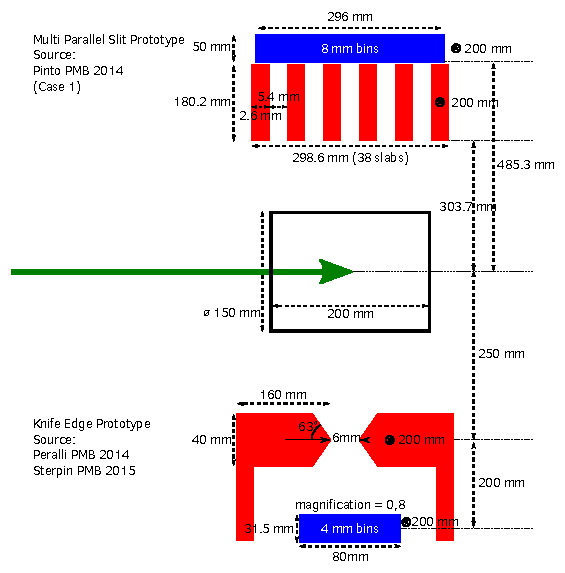
\includegraphics[width=\textwidth]{./figures/detectors_cyl}
						\caption{Prototypes representation}
						\label{CamerasScheme}
					\end{figure}					
				\end{column}				

			\end{columns}

	  \end{block}		  
	\end{column} % end of left column
	
	\begin{column}{0.49\textwidth} % right column
	  \vspace{-2ex}
		
		
		
		\begin{block}{6. Figures of merit\label{FOM}}
			
			\begin{itemize}
				\item Detection efficiency (DE): \#detected PG/\#emitted PG in the camera Field of View
				\item Spatial resolution (Res) = FOW (Fall-Off Width)
				\item Fall-off Retrieval Precision (FRP): Standard deviation of the FOP distribution obtained with 50 MC simulation runs.
			\end{itemize}


	  \end{block}				
		

       
	  %%%%%%%%%%%%%%%%%%%%%%%%%%%%%%%%%%%%%%%%%%%%%%%%%%%%%%  
		
		\begin{block}{7. Results}
			{\Red{\large{AMV}}}
			\begin{table}[h]
			\centering
			\begin{tabular}{llllll}
				\midrule
							& \multicolumn{2}{c}{MPS}												&& \multicolumn{2}{c}{KES}										\\
				\cline{2-3}\cline{5-6}
							& AM 											& MC 									&& AM 										& MC								\\
				\midrule

				FOW (mm)& 14.5 								& 16.9  	 					&& 13.5 								& 13.8 						\\
				DE		& $6.66 \times 10^{-4}$  & $6.47 \times 10^{-4}$	&&	$1.06 \times 10^{-3}$   & $8.7 \times 10^{-4}$\\
				\midrule
			\end{tabular}
			\end{table}			
			{\Red{\large{PG profiles detected by the prototypes}}}
% 			\begin{columns}[t]
% 
% 				\begin{column}{0.49\textwidth}			
% 					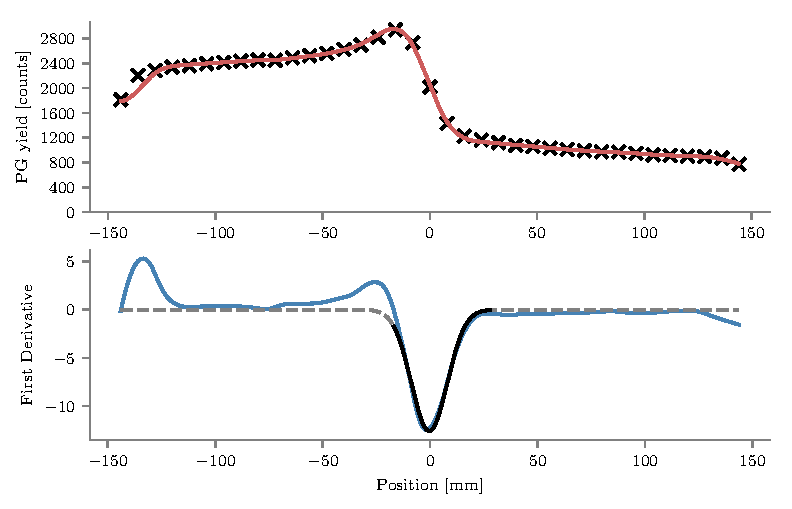
\includegraphics[width=\textwidth]{./figures/PMMA_phantom-ipnl-auger-notof-1}
% 				
% 				\end{column}			
% 
% 				\begin{column}{0.49\textwidth}
% % 					\begin{figure}
% 						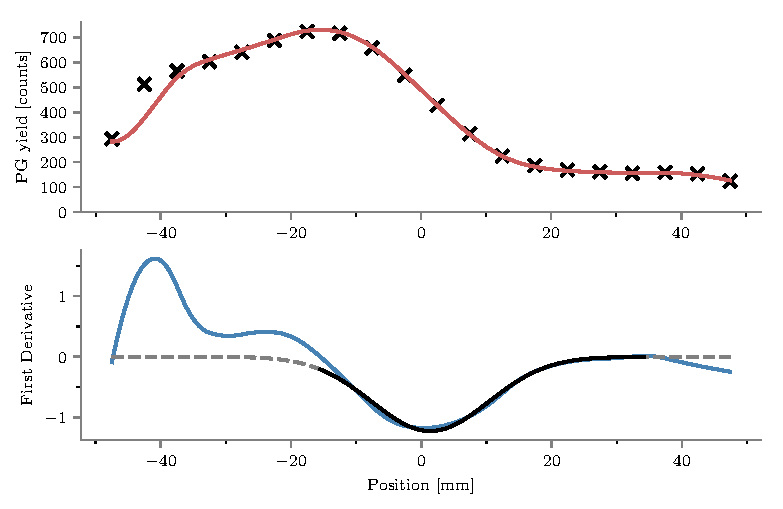
\includegraphics[width=\textwidth]{./figures/PMMA_phantom-iba-auger-notof-3}			
% % 						\caption{\hl{Change the target diameter: 15 cm}}
% % 						\label{CamerasScheme}
% % 					\end{figure}					
% 				\end{column}				

% 			\end{columns}
			
				\begin{figure}
					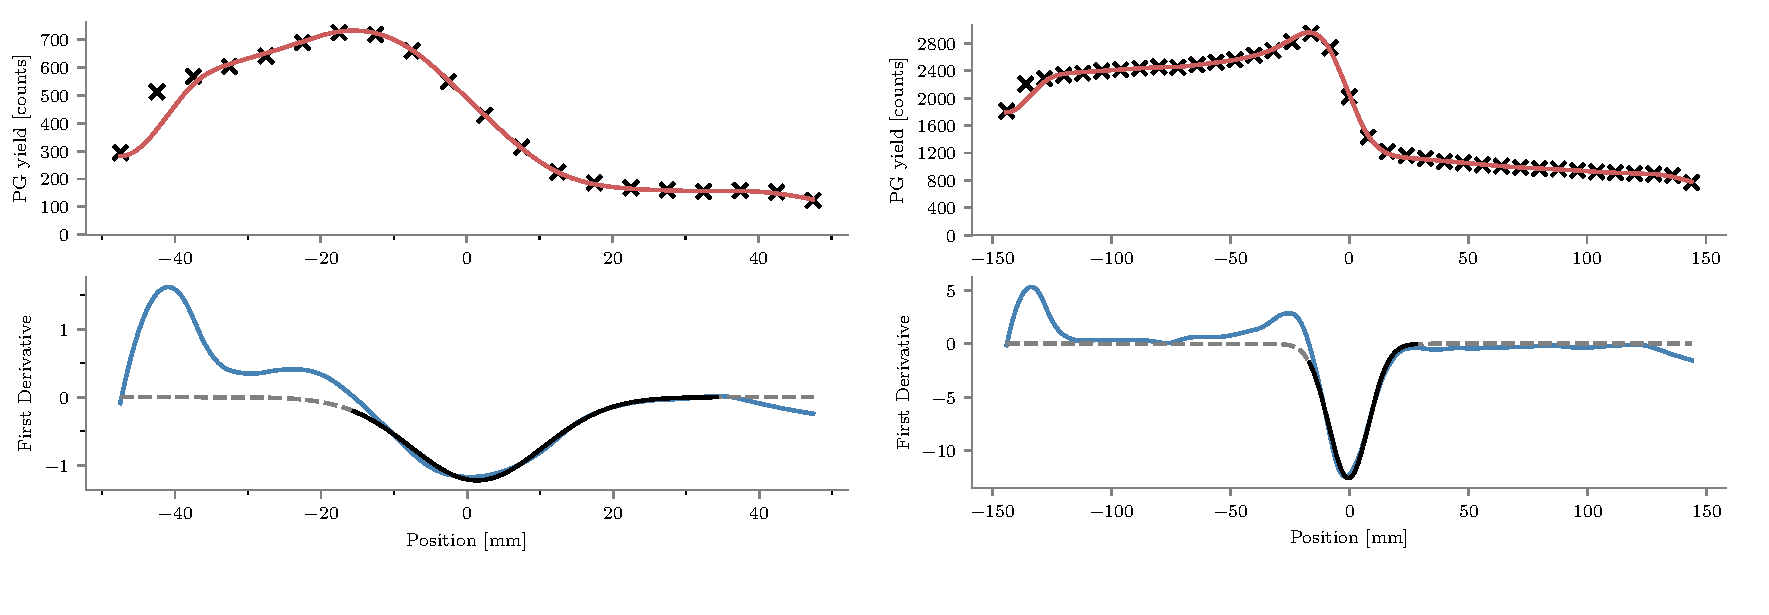
\includegraphics[width=\textwidth]{./figures/output-crop}			
					\caption{Top: PG profiles obtained with MPS (left) and KES (right). See column PC of Table~\ref{CamerasParameters} for the parameters. Bottom: first derivative of the PG profiles.}
					\label{PGprofiles}
				\end{figure}					
				
				
			{\Red{\large{Fall-off Retrieval Precision}}}
% 			\begin{table}[h]
% 			\centering
% 			\begin{tabular}{llllllllllll}
% 				\midrule
% 				Time selection 					& \mc{5}{c}{ToF} &   &  \mc{5}{c}{None}     \\
% 				\cline{2-6}\cline{8-12}
% 				Energy selection (MeV) 	& \mc{2}{c}{$>1$}    & & \mc{2}{c}{3--6}   & &  \mc{2}{c}{$>1$}    & & \mc{2}{c}{3--6}    \\
% 				\cline{2-3}\cline{5-6}\cline{8-9}\cline{11-12}
% 				Camera 						& MPS & KES && MPS & KES & & MPS & KES && MPS & KES \\
% 				\midrule
% 				$10^9$ (\# protons)& \textbf{0.37} & 0.55 && 0.44 & 1.07 && 0.42 & 0.74 && 0.66 & \textbf{1.32} \\
% 				$10^8$    				& \textbf{1.35} & 2.08 && 1.60 & 4.22 && 1.36 & 1.82 && 2.00 & \textbf{9.70} \\
% 				$10^7$    				& \textbf{4.41} & 11.88 && 20.36 & 20.50 && 22.45 & 17.18 && 56.92 & \textbf{19.39} \\
% 				\midrule
% 			\end{tabular}
% 			\caption{\tcr{TO VERIFY: Standard deviation of the FOP distribution}. In bold, the cuts and ToF selections as proposed.}
% 			\label{FRPCOMP}
% 			\end{table}			
			\begin{table}[h]
			\centering
			\begin{tabular}{lccccccc}
				\midrule
				\# protons & \multicolumn{3}{c}{MPS} && \multicolumn{3}{c}{KES} \\
				%\cline{2-3}\cline{5-6}
				& FRP & FOW & DE && FRP & FOW & DE\\
				\midrule
				$10^9$ & $0.32$ & $19.4$ & $1.04\times10^{-3}$ && $0.65$ & $20.1$ & $5.58\times10^{-4}$\\
				$10^8$ & $1.05$ & $19.4$ & $$ && $1.80$ & $20.1$ & $$\\
				$10^7$ & $2.81$ & $19.4$ & $$ && $17.1$ & $20.1$ & $$\\
				\midrule
			\end{tabular}
			\caption{Standard deviations (in mm) of the FOP distributions. See column PC of Table~\ref{CamerasParameters} for the parameters.}
			\label{FRPCOMP}
			\end{table}					
		\end{block}

	\begin{block}{8. Discussion and conclusion}	
		\begin{itemize}
			\item Analytical Model (AM)
			\begin{itemize}
				\item Good agreement in overall with MC
				\item Striking similarities between MPS and KES performances, unlike what can be concluded from previous studies \cite{Smeets2016,Lin2016,Park2019} 
				\begin{itemize}
					\item[$\Rightarrow$] Same DE and FOW with perfect collimators	
					\item[$\Rightarrow$] With real collimators: slightly poorer DE for MPS and FOW for KES 
					\item Note that the MPS prototype allows for the detection of the whole PG profile: the field of view of the MPS and KES prototypes are of 30~cm and 10~cm, respectively
				\end{itemize}			
			\end{itemize}

			\item Prototypes comparison
			\begin{itemize}
				\item PG profiles: MPS prototype with larger fall-off amplitude and lower BKG level thanks to wider energy selection and TOF selection, respectively
				\item[$\Rightarrow$] Better Fall-Off Retrieval Precision (FRP) with the MPS	prototype
				\item Precisions in agreement with the ones published in \cite{Pinto2014} and \cite{Smeets2012}
			\end{itemize}			

		\end{itemize}

		
		
	\end{block}

		
			  %%%%%%%%%%%%%%%%%%%%%%%%%%%%%%%%%%%%%%%%%%%%%%%%%%%%%% 
	  \begin{block}{References}
	    \tiny
% 			\begin{spacing}{0.5}
	    \setbeamertemplate{bibliography item}[text] 
%	    \bibliographystyle{elsarticle-num}
	    \bibliographystyle{ieeetr}
	    \bibliography{biblio_abb}				
% 			\end{spacing}


	  \end{block}		
		

	  
	  \vfill
	  
	\end{column}
	
\end{columns}

      
\end{frame}
\end{document}
